\documentclass[11pt,twocolumn]{article}
\usepackage[utf8]{inputenc}
\usepackage[T1]{fontenc}
\usepackage{graphicx}
\usepackage{amsmath}
\usepackage{hyperref}
\graphicspath{{figures/}}

\title{RATISS-Cyber : Détection d'intrusion par topologie\\
des transitions de phase}
\author{Anonyme --- SMI CybIA 2026, Douala}
\date{}

\begin{document}
\maketitle

\begin{abstract}
Les détecteurs d'intrusion classiques analysent les \emph{symptômes}
statistiques du trafic. Nous montrons qu'une classe d'attaques furtives,
construites pour être \emph{statistiquement invisibles} (tests de
Kolmogorov-Smirnov : $\geq 90\%$ des features indistinguables du normal),
échappe à ces détecteurs mais trahit sa présence par la \emph{structure} de
ses corrélations. En adaptant l'arsenal de la physique des transitions de
phase topologiques (homologie persistante, participation ratio spectral,
mécanisme de Kibble-Zurek, frustration de triades), nous construisons une
batterie d'observables structurelles. Sur un dataset synthétique contrôlé,
chaque attaque est détectée par son observable propre : le participation
ratio détecte la transition de phase (rappel $0.95$ vs $0.67$ classique), le
cumul de Kibble-Zurek détecte le tissage ($0.79$ vs $0.07$). Une fusion
spécialisée par famille atteint un rappel moyen de $0.61$ à $1.7\%$ de faux
positifs --- $2.3\times$ le classique seul. Chaque alerte embarque une preuve
SHA-256 vérifiable.
\end{abstract}

\section{Introduction}
Les systèmes de détection d'intrusion (IDS) reposent sur des signatures
statistiques du trafic : distributions, volumes, fréquences. Or un attaquant
sophistiqué peut \emph{préserver les marginales} tout en réorganisant la
\emph{structure} des dépendances entre features. Nous formalisons trois
familles d'attaques de ce type et montrons que ces réorganisations sont des
\textbf{transitions de phase} au sens physique, détectables par les outils de
la matière condensée topologique.

\textbf{Contributions.} (1) Trois attaques garanties statistiquement
invisibles (tests KS). (2) Une batterie d'observables topologiques adaptées
de la physique des transitions. (3) Une fusion spécialisée par famille
atteignant un rappel moyen de $0.61$ à FPR $1.7\%$. (4) Une preuve SHA-256
vérifiable par alerte.

\section{Menaces : attaques statistiquement invisibles}
Trois familles, garanties invisibles par tests KS (Tableau~\ref{tab:ks}) :

\textbf{Tissage.} Inversion du signe d'un tiers des corrélations --- le motif
change, la moyenne reste (analogie : cristal photo-induit KTN:Li).

\textbf{Transition de phase.} Bascule d'une structure en blocs indépendants
vers un hub centralisé (analogie : modèle SSH).

\textbf{Mutation lente (APT).} Dérive progressive --- chaque fenêtre est
normale, la trajectoire est anormale (analogie : Kibble-Zurek).

\begin{table}
\centering
\caption{Invisibilité statistique (tests KS)}
\label{tab:ks}
\begin{tabular}{@{}lc@{}}
\hline
Attaque & Features indistinguables \\
\hline
Tissage & $16/16 \geq 90\%$ \\
Transition de phase & $15/16$ \\
Mutation lente & $16/16$ \\
\hline
\end{tabular}
\end{table}

\section{Observables topologiques}
\begin{table}
\centering
\caption{Batterie d'observables structurelles}
\label{tab:obs}
\begin{tabular}{@{}lll@{}}
\hline
Observable & Mesure & Source physique \\
\hline
P\_sig & boucles H1 & persistance Vietoris-Rips \\
PR & délocalisation spectrale & participation ratio \\
KZ cumul & dérive directionnelle & mécanisme de Kibble-Zurek \\
Frustration & triangles frustrés & verre de spin / KTN:Li \\
Edge & poids extrémal & concentration des corrélations \\
Drift & trajectoire & dérive entre fenêtres \\
\hline
\end{tabular}
\end{table}

\section{Résultats}
\textbf{Chaque attaque a son observable.} La
Figure~\ref{fig:canal} montre que le classique plafonne là où l'observable
adapté voit la structure.

\begin{figure}[t]
\centering
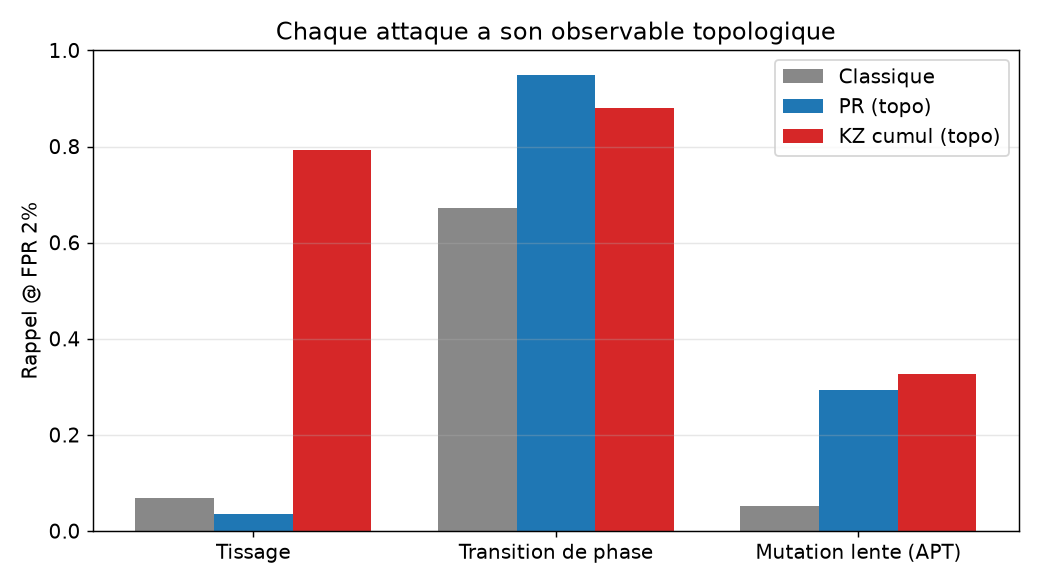
\includegraphics[width=\columnwidth]{fig1_rappel_par_canal.png}
\caption{Rappel par canal et par famille @ FPR 2\%.}
\label{fig:canal}
\end{figure}

\textbf{Délocalisation spectrale.} La transition de phase fait monter le PR
($7.6 \to 9.5$, Figure~\ref{fig:pr}).

\begin{figure}[t]
\centering
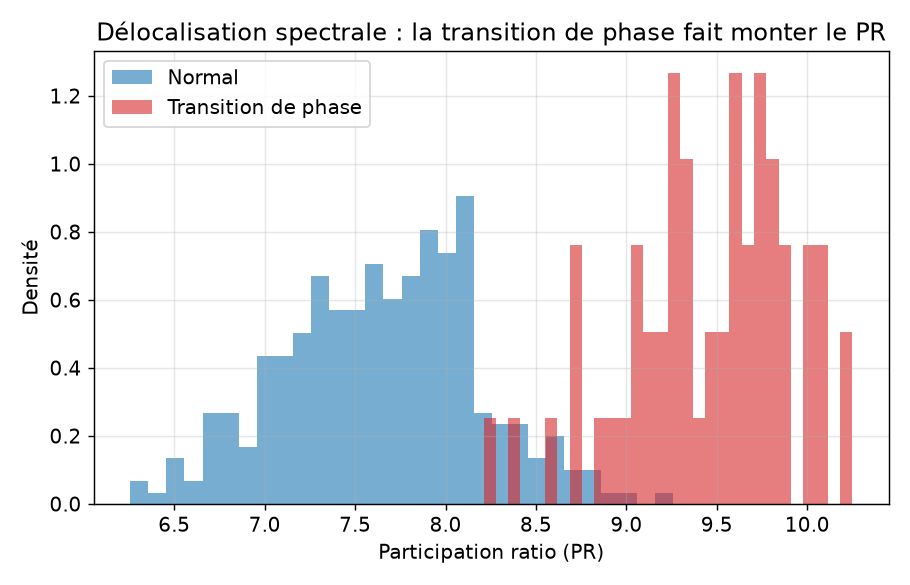
\includegraphics[width=\columnwidth]{fig2_pr_transition.png}
\caption{Distribution du participation ratio : normal vs transition de phase.}
\label{fig:pr}
\end{figure}

\textbf{Dérive structurelle.} Le cumul de Kibble-Zurek s'élève sous attaque
(Figure~\ref{fig:kz}).

\begin{figure}[t]
\centering
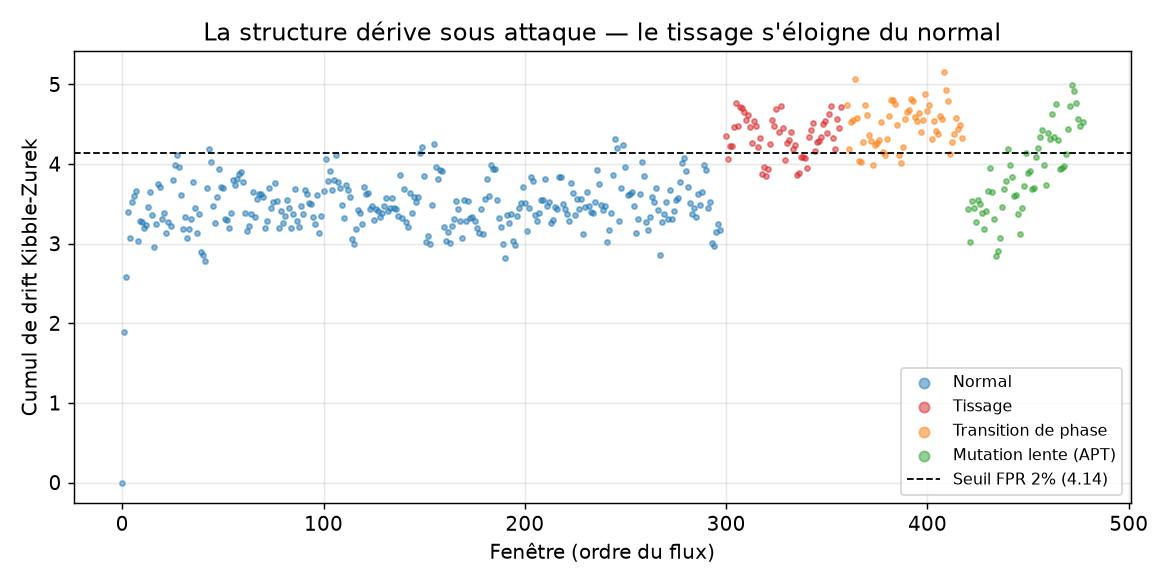
\includegraphics[width=\columnwidth]{fig3_trajectoire_kz.png}
\caption{Trajectoire Kibble-Zurek le long du flux.}
\label{fig:kz}
\end{figure}

\begin{figure}[t]
\centering
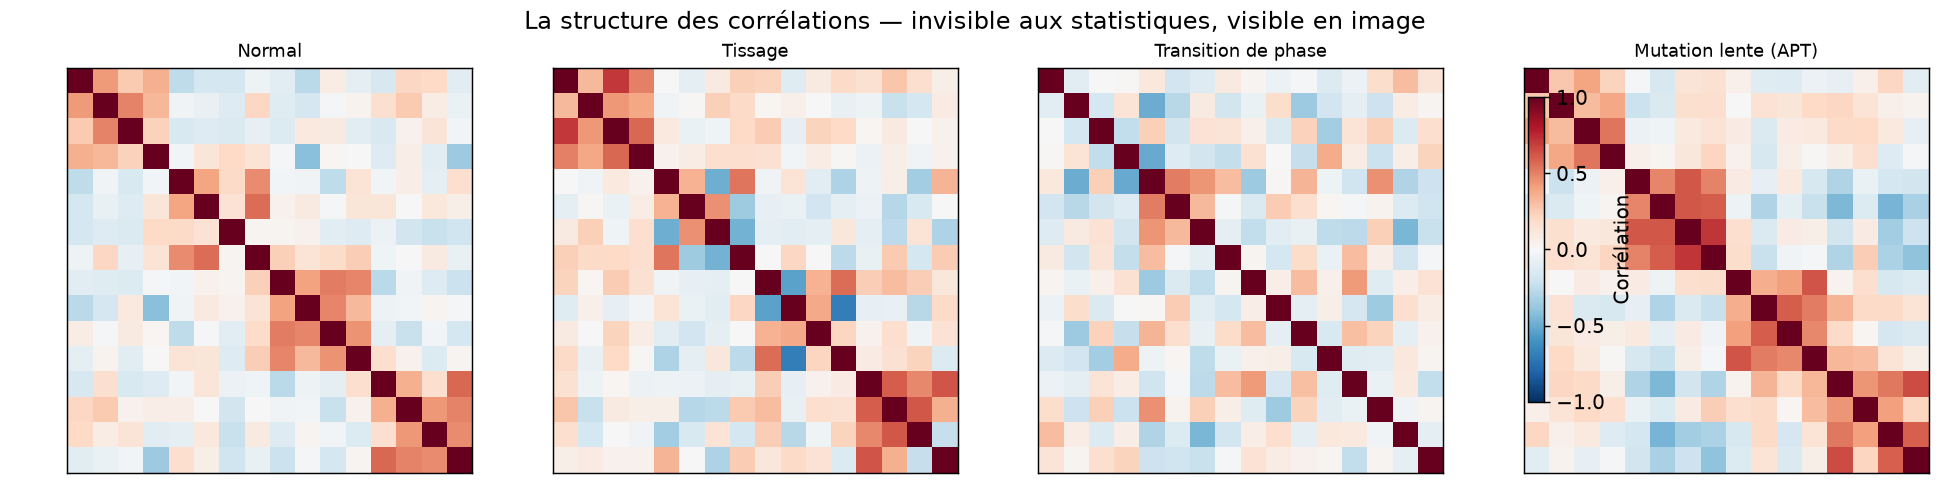
\includegraphics[width=\columnwidth]{fig4_matrices_correlation.png}
\caption{Matrices de corrélation : la structure visible.}
\label{fig:mat}
\end{figure}

\textbf{Fusion par famille.} Sélection automatique du meilleur canal par
famille, orchestrateur par OU logique. Rappel moyen $0.61$ à FPR global
$1.7\%$ --- contre $0.26$ pour le classique seul.

\begin{table}
\centering
\caption{Rappel par famille (fusion spécialisée)}
\label{tab:res}
\begin{tabular}{@{}lll@{}}
\hline
Famille & Canal & Rappel \\
\hline
Tissage & KZ cumul & $0.67$ \\
Transition de phase & PR & $0.90$ \\
Mutation lente & KZ cumul & $0.28$ \\
\hline
\end{tabular}
\end{table}

\section{Limites et travaux futurs}
Le cumul KZ détecte les campagnes groupées (pas les attaques isolées) ; la
mutation lente reste la plus difficile ; la validation sur trafic réel
(CIC-IDS2017) et la LCT (Learning-Coupled Topology) pour l'adaptation
continue sont en cours.

\section{Conclusion}
La cybersécurité gagne à regarder le trafic comme un système physique : les
intrusions furtives sont des transitions de phase, et l'arsenal de la matière
condensée topologique les rend visibles.

\end{document}
